\chapter{Quantum technologies}

This chapter will provide a brief overview of the current state-of-the-art in quantum technological advances. This will not only give us insights in how the technology is being used today, but also grant us the opportunity to discuss key concepts that are fundamental to understand for this thesis. Thereafter we will look into how materials are composed, and what kind of properties a material needs to exhibit to be an eligible host for quantum devices. Finally, we will giving a few specific examples of materials with promising point defects that have been comprehensively researched. Importantly, this will motivate the reasoning for finding new materials that might excel in areas where other materials falls short for utilization in quantum technology.

\textit{Quantum technology} (QT) refers to practical applications and devices that utilize the principles of quantum physics as a foundation. Technologies in this spectrum are based on concepts such as \textit{superposition}, \textit{entanglement} and \textit{coherence}, which are all closely related to one another.

A quantum superposition refers to that any two or more quantum eigenstates can be added together into another valid quantum state, such that every quantum state can be represented as a sum, or a superposition, of two or more distinct states. This is according to the wave-particle duality which states that every particle or another quantum entity may be described as either a particle or a wave. When measuring the state of a system residing in a superposition of eigenstates, however, the system falls back to one of the basis states that formed the superposition, destroying the original configuration.

Quantum entanglement refers to when a two- or many-particle state cannot be expressed independently of the state of the other particles, even when the particles are separated by a significant distance. As a result, the many-particle state is termed an entangled state \cite{Griffiths2017}.

Quantum coherence arises if two waves coherently interfere with each other and generate a superposition of the two states with a phase relation. Likewise, loss of coherence is known as \textit{decoherence}.

%The terms superposition, entanglement and coherence are closely related. The two latter terms are the primary features of quantum mechanics that are lacking in classical mechanics, giving rise to paradoxes such as Einstein's famous Schrödingers cat, which is both dead and alive at the same time when in its coherent state inside a closed box.

Another concept that the reader should be familiar with is the famous Heisenberg uncertainty principle. It states that
\begin{align}
    \sigma_x \sigma_p \leq \frac{\hslash}{2},
    \label{eq:uncertainty}
\end{align}
where $\sigma_x$ is the standard deviation for the position and $\sigma_p$ is the standard deviation in momentum. This means that we cannot accurately predict both the position and momentum of a particle at the same time. Thus, we often calculate the probability for a particle to be in a state which results in concepts such as an electron sky surrounding an atom core. However, remember that equation (\ref{eq:uncertainty}) is an inequality, which means that it is possible to create a state where neither the position nor the momentum is well defined.

\section{Quantum computing}
%The evolution of the digital worlds computational powers is a remarkable piece of history
The start of the digital world's computational powers can be credited to Alan Turing. In 1937, Turing \cite{Turing1937} published a paper where he described the \textit{Turing machine}, which is regarded as the foundation of computation and computer science. It states that only the simplest form of calculus, such as boolean Algebra ($1$ for true and $0$ for false), is actually computable. This required developing hardware that could handle classical logic operations, and was the basis of transistors that are either in the state ON or OFF depending on the electrical signal. Equipped with a circuit consisting of wires and transistors, commonly known as a computer, we could develop software to solve all kinds of possible applications.

Driven by the development of software, conventional computers have in accordance to Moore's law \cite{Moore1965}, doubled the amount of transistors on integrated circuit chips every two years as a result of smaller transistors. Furthermore, the clock frequency has enhanced with time, resulting in a doubling of computer performance every 18 months \cite{Pavicic2006}. Alas, miniaturization cannot go on forever as transistors are mass-produced at $5$ nm today and are expected to reach a critical limit of $3$ nm in the following years \cite{Gwennap2020}.

To sustain the digital world's increasing computational demand, other alternatives than the conventional classical computer must be explored. This is where quantum computing comes into the picture. The term quantum computer is a device that exploits quantum properties to solve certain computational problems more efficiently than allowed by Boolean logic \cite{Weber2010}.

The idea is to pass information in the form of a quantum bit, or \textit{qubit} for short. They are the building blocks of quantum computers, and as opposed to the conventional $0$ or $1$-bits that classical computers are based on, they can inhabit any superposition of the states $0$ or $1$. This is illustrated in figure \ref{fig:qubit and bit}.

%Since a qubit has a quantum nature and is the counterpart to the classical bit, it naturally follows that it is in the center of attention in quantum computation\footnote{There exists other systems such as the quantum d-state system, known as \textit{qudits}, that can also be utilised in quantum computation \cite{Ladd2010}.}.

The architecture of a gate-based quantum computer is dependent on a set of quantum logic gates that perform unitary transformations on sets of qubits \cite{DiVincenzo2000, Ladd2010}. A different implementation of quantum computers exists is adiabatic quantum computer. This approach is not based on gates, but on defining the answer of a problem as the ground state of a complex network of interactions between qubits, and then controlling the interactions to adiabatically evolve the system to the ground state \cite{Mizel2007}.

\begin{wrapfigure}{r}{0.5\textwidth}
  \centering
  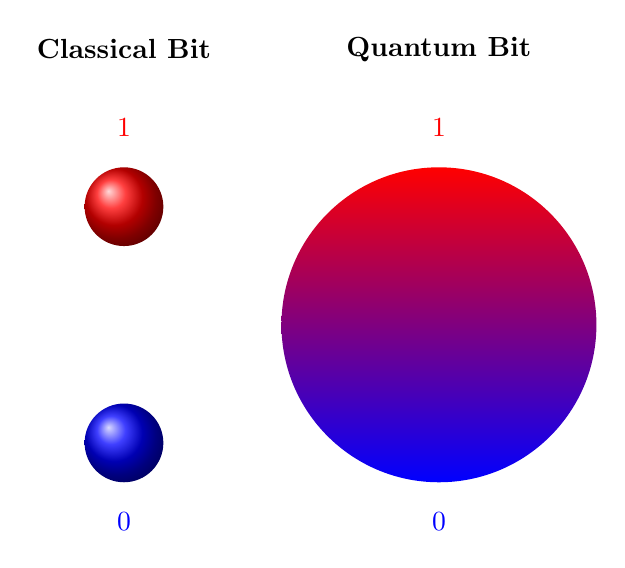
\begin{tikzpicture}[scale=1]
    \node[font=\bfseries] at (0,2) {Classical Bit};
    \node[font=\bfseries] at (4,2) {Quantum Bit};

    \node[color=red] at (0,1) {$1$};
    \node[color=blue] at (0,-4) {$0$};

    \node[shade,shading=ball,circle,ball color=blue,minimum size=1cm] (ball) at (0,-3) {};
    \node[shade,shading=ball,circle,ball color=red,minimum size=1cm] (ball) at (0,0) {};

    \node[color=red] at (4,1) {$1$};
    \node[color=blue] at (4,-4) {$0$};
    \node[shade, shading=ball,circle,top color=red, bottom color=blue, minimum size=4cm] (ball) at (4,-1.5) {};
  \end{tikzpicture}
  \caption{Conceptual illustration of the two-level classical bit, which are restricted to the boolean states 1 (true) or 0 (false), and the quantum bit that can be in any superposition of the states 0 or 1.}
  \label{fig:qubit and bit}
\end{wrapfigure}


It has been demonstrated that exponentially complex problems can be reduced to polynomially complex problems for quantum computers \cite{Pavicic2006}. For example, a quantum search algorithm found by Grover \cite{Grover1997} offers a quadratic speed-up compared to classical algorithms, while Shor's quantum integer factorization algorithm \cite{Shor1994} presents an exponential speed-up. Intriguingly, Google reported in $2019$ that they ran a random number generator algorithm on a superconducting processor containing 53 qubits in $200$ seconds, which would most likely take several times longer for a classical supercomputer to solve \cite{Martinis2019}. It is anticipated that quantum computers will excel in exceedingly complex problems, while many simpler tasks may not see any speed-up at all compared to the classical regime. Hence, quantum- and classical computers are envisioned to coexist to utilize the strength of each technology.

%However, it is not to avoid that both quantum  hardware and -software is in its preliminary phase of development, and it will be interesting to follow up the progression the following years.

Quantum computing is a highly sought-after goal, but there are extensive challenges that needs to be adressed. Controlling a complex many-qubit system is difficult, since it is not always possible to establish interactions between qubits \cite{DiVincenzo2000} and maintain entaglement over both time and distance. Additionally, decoherence and other quantum noise occurs as a result of the high volatility of quantum states, making quantum state manipulation prone to errors. The \textit{quantum error correction} protocols and the theory of \textit{threshold theorem} deals with this vulnerability, stating that noise most likely does not pose any fundamental barrier to the performance of large-scale computations \cite{Pavicic2006}.


\subsection{Quantum computing requirements}
As ever-promising the concepts of quantum technology are, the physical realizations are in the preliminary stage of development. Here we will concretize critical principles for a physical realisation of a quantum platform.

\begin{quote}
   ``I always said that in some sense, these criteria are exactly the ones that you would teach to kindergarten children about computers, quantum or otherwise'' DiVincenzo \cite{Georgescu2020}
\end{quote}

\noindent DiVincenzo formulated in the year of $2000$ seven basic criteria for a physical qubit system with a logic-based architecture \cite{DiVincenzo2000}.

\begin{enumerate}
  \item A scalable physical system with well characterized qubits
  \item The ability to initialize the state of the qubits to a simple initial system
  \item Have coherence times that are much longer than the gate operation time
  \item Have a universal set of quantum gates
  \item Have the ability to perform qubit-specific measurements
  %\item The ability to convert stationary qubits to flying qubits
  %\item The ability to faithfully transmit flying qubits between specified locations
\end{enumerate}

\noindent These five criteria must be met for a quantum platform to be considered a quantum computer.

%The first five criteria (1-5) must be met for a quantum platform to be considered a quantum computer, while the two last criteria (6-7) were added for quantum communication, since its applications provide a unique advantage compared to its classical counterpart.


%Quantum hardware and -software are both in the preliminary stage of development, and it will be interesting to follow their progress the following years.

\section{Quantum communication}

Quantum communication refers to the transfer of a state of one quantum system to another. Since information can be stored in qubits, we picture \textit{flying qubits} that transfer information from one location to another \cite{Griffiths2002}. The benefits of using flying qubits are in particular valued in quantum cryptography, since the quantum nature of qubits can be exploited to add extra layers of security \cite{Pavicic2006}.

%as it is regarding \textit{flying qubits} , a photon carrying a quantum state, which is an example of a \textit{flying qubit}.

%A significant portion of quantum communication is also part of other quantum information theories such as quantum cryptography, which comes as a remedy to a rising paranoia concerning security \cite{Griffiths2002, Pavicic2006}.

%Classical cryptography encrypts information with the use of a key.
Consider the example of encrypting a digitally transmitted conversation. It is difficult to avoid someone eavesdropping on a conversatio. However, the problem is diminished if the eavesdropper does not speak the language, keeping the information in the conversation safe. This is the original idea of encryption, such that the information has been encrypted into something incomprehensible for any eavesdropper. A common practice is to encrypt information and share a public key, which everyone can read, and a private key, only known for the sender and receiver of information. This should be sufficient to keep the information secure, given that the complexity of the private key is impenetrable.

Importantly, we live in a digital world where most of our actions are increasingly being stored as information, and we could imagine that the eavesdropper in the latter example stored the conversation. Even if the content of the conversation was encrypted, it still presents a challenge, since encrypted information stored today could be deciphered in ten or twenty years' time
%\footnote{As an example, in Martin Gardner's \textit{Scientific American} column in $1976$ \cite{Taubes1994}, the $129$-digit RSA key was thought to be safe for $5000$ mips (million instructions per second) years, equal to $4 \times 10^{25}$ years. Only $17$ years later, the factorization was a reality and the public key was revealed to be ``The Magic Words are Squeamish Ossifrage'' \cite{Atkins1995}. To compare to todays fastest supercomputer Fugaku \cite{Top500} by making two \textit{very} rough estimations that flops and mips are approximately the same in addition to solely basing the calculation on computing power, the $129$-digit RSA private key would be found in less than half a second using Fugaku.}
. Consequently, finding an encryption method that could make information either impossible to eavesdrop on or make the security unbreakable forever is very desirable. This is the ultimate goal of quantum cryptography \cite{Pavicic2006}.

Consider the example of information encoded into a qubit as a superposition of two quantum states. Now, if a wild eavesdropper would try to measure the information, the nature of quantum physics tells us that the original configuration would be destroyed and the receiver would be alerted of the eavesdropper. Furthermore, if the eavesdropper would try to make a copy of the message, the copying itself would be limited of the no-cloning theorem \cite{Gisin2002} which declare that quantum states cannot be copied.

A clever approach to ensure confidentiality is to send the encryption key before sending the actual encrypted information. If the key is received unperturbed, the key remains secret and can be safely employed. If it turns out perturbed, confidentiality is still intact since the key does not contain any information and can be discarded. This approach is termed the \textit{quantum key distribution} (QKD) \cite{Gisin2002, Gisin2007}. It should be noted that this requires both the sender and receiver to have access to methods for sending, receiving and storing qubit states, such as a quantum computer. Additionally, the sender and receiver will need to initially exchange a common secret which is later expanded, making quantum key \textit{expansion} a more exact term for QKD \cite{Pavicic2006, Gisin2007}.

Most applications and experiments use optical fibers for sending information via photons, with the distance regarded as the main limitation. This is because classical repeaters are unable to enhance quantum information because of the no-cloning theorem, making photon loss in optical fiber cables inevitable. Thus, quantum communication must reinvent the repeater concept, using hardware that preserves the quantum nature \cite{Acin2018} and are compatible with wavelengths used in telecommunication. Nonetheless, secure QKD up to $400$ km has recently been demonstrated using optical fibres in academic prototypes \cite{Boaron2018}.

\section{Quantum sensing}

Measurements are part of our digital world today to a great extent. There would be no way to exchange goods, services or information without reliable and precise measurements \cite{Acin2018}. Thus, improving the accuracy of sensors for all types of measurements is desirable. One potential method to improve measurement accuracy, resolution and sensitivity is utilizing quantum sensors. Quantum sensors exploit quantum properties to measure a physical quantity \cite{Degen2017}. This is possible because quantum systems are highly susceptible to pertubations to its surroundings, and can be used to detect physical properties such as either temperature or an electrical or magnetic field \cite{Degen2017}.

For a quantum system to be able to function as a quantum sensors, a few criterias needs to be met.  Firstly, the quantum system needs to have discrete and resolvable energy levels. The quantum system also needs to be controllably initialised into a state that can be identified and coherently manipulated by time-dependent fields. Lastly, the quantum system needs to be able to interact with the physical property one wants to measure through a coupling parameter \cite{Degen2017}.

It is also possible to also exploit quantum entanglement to improve the precision of a measurement. This gain of precision is used to reach what is called the Heisenberg-limit, which states that the precision scales as the number of particles $N$ in an idealized quantum system \cite{Degen2017, Acin2018}, while the best classical sensors scale with $\sqrt{N}$.

\section{Available quantum platforms}

%Before a quantum system can be used in either quantum computing, quantum cryptography or quantum sensing, a few criterias has to be met. They are formulated by

Many different quantum platforms have been physically implemented, and this section will serve as a brief overview of the current status. For a more thorough review of qubit implementations, the reader is directed to Refs. \cite{Ladd2010, Acin2018}. \\

Superconducting circuits can be used in quantum computing, since electrons in superconducting materials can form Cooper pairs via an effective electron-electron attraction when the temperature is lower than a critical limit. Below the limit, electrons can move without resistance in the material \cite{KristianFossheim2004}. Exploiting this intrinsic coherence, qubits can be made by forming microwave circuits based on loops of two superconducting elements separated by an insulator, also known as Josephson tunnel junctions \cite{Acin2018}. Today, superconducting Josephson junctions are the most widely used quantum platform, but they requires very low temperature (mK) to function, making them costly to use. Additionally, the current devices experience a relatively short coherence time, causing challenges in scaling up. \\

Single photons is an eligible quantum platform that can be implemented as qubits with one-qubit gates being formed by rotations of the photon polarization. Its use in fiber optics are less prone to decoherence, but faces challenges since the more complex photon-photon entanglement and control of multi-qubits is strenuous \cite{Ladd2010}. \\

By fixing the nuclear spin of solid-state systems, it is possible to implement a quantum platform that experience long spin coherence. This enables the manipulation of qubits that utilize electromagnetic fields, making one-qubit gates realizable. \\

The isolated atom platform is characterized by its well-defined atom isolation. Here, every qubit is based on energy levels of a trapped ion or atom. Quantum entanglement can be achieved through laser-induced spin coupling, however scaling up to large atom numbers induce problems in controlling large systems and cooling of the trapped atoms or ions. \\

A quantum dot (QD) can be imagined as an artifical atom which is confined in a solid-state host. As an example, a quantum dot can occur when a hole or an electron is trapped in the localized potential of a semiconductor's nanostructure. QDs exhibit similar coherence potential as the isolated atom platform, but without the drawback of confining and cooling of the given atom or ion \cite{Acin2018}. Moreover, it is possible to limit decoherence due to nuclear spins by dynamic decoupling of nuclear spin noise and isotope purification \cite{Ladd2010}.

A QD can normally be defined litographically using metallic gates, or as self-assembled QDs where a growth process creates the potential that traps electrons or holes. The difference between them is a question of controllability and temperature, since the metallic gates is primarily controlled electrically and operate at $<1$ K, while self-assembly QDs are primarily controlled optically at $\sim 4$ K \cite{Ladd2010}. Despite requiring very low temperatures, QDs have the potential for fast voltage control and opticial initialization. As with trapped ions, electrostatically defined quantum dots experience a short-range exchange interaction, imposing a limitation for quantum computing and quantum error correction protocols. A potential solution could include photonic connections between quantum dots. Indeed, self-assembled quantum dots couple strongly to photons due to their large size in comparison to single atoms. However, the size and shapes of self-assembled quantum dots are decided randomly during the growth process, causing an unfavourable large range of optical absorption and emission energies \cite{Ladd2010}.



%In such a system, the spin degree of freedom is considered favourable due to its long coherence time \cite{Acin2018}.

Lastly, we will turn towards point defects in bulk semiconductors as a physical implementation of a quantum platform. Point defects shares many of the attributes of quantum dots, such as discrete optical transitions and controllable coherent spin states. %but are vulnerable to small changes in the lattice of the semiconductor.
Depending on the semiconductor host and the defect system of interest, they may exhibit extended coherence times and greater optical homogeneity than other quantum dot systems. Before we dwell into the intricacies of point defect qubits as a building block for QT, we will provide the neccessary background for the crystal- and electronic structure of semiconductors.   %Thus, we will hereafter focus our attention on qubit host candidates.

\section{Introduction to semiconductor physics}

The interactions between atoms and the resulting characteristics of matter form the foundation of materials science. The applications of materials science are extensive, with examples such as a bottle of water or to a chair to sit in.

\begin{figure}[ht!]
  \centering
\begin{subfigure}{.5\linewidth}
\centering
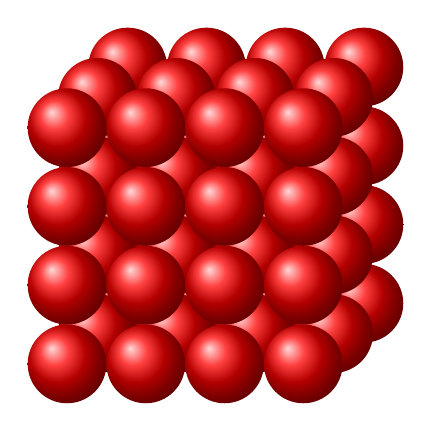
\begin{tikzpicture}
  \foreach \z in {1,2,3}{
  \foreach \i in {3,2,1,0}{% This one doesn't matter
    \foreach \j in {3,2,1,0}{% This will crate a membrane
        \shade[ball color=red] ({\i},{\j},\z) circle(0.5);
      }
    }
  }
\end{tikzpicture}
\subcaption{} \label{fig:M1}
\end{subfigure}%
\par\bigskip

\begin{subfigure}{1.0\linewidth}
\centering
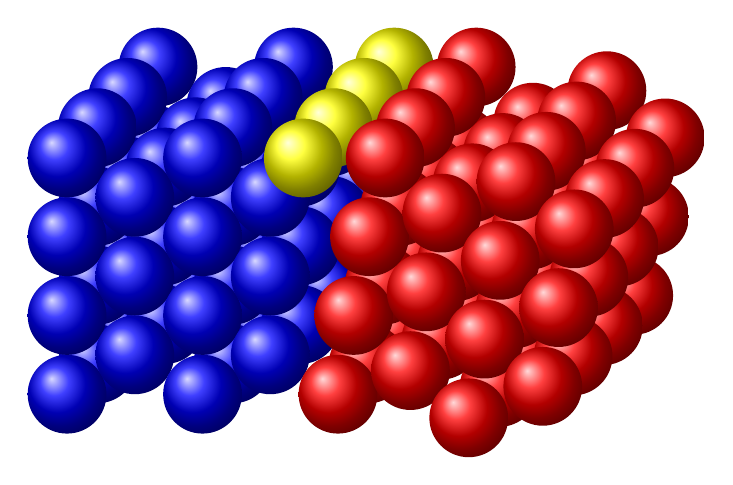
\begin{tikzpicture}
    \foreach \x in {0,1,2,3}{%
      \foreach \z in {0,1,2,3}{%
      \shade[ball color=blue] (0,\x,\z) circle(0.5);
      }
    }
    \foreach \x in {0.5,1.5,2.5}{%
      \foreach \z in {0,1,2,3}{%
      \shade[ball color=blue] ({1*sqrt(0.74)},\x,\z) circle(0.5);
      }
    }
    \foreach \x in {0,1,2,3}{%
      \foreach \z in {0,1,2,3}{%
      \shade[ball color=blue] ({2*sqrt(0.74)},\x,\z) circle(0.5);
      }
    }
    \foreach \x in {0.5,1.5,2.5}{%
      \foreach \z in {0,1,2,3}{%
      \shade[ball color=blue] ({3*sqrt(0.74)},\x,\z) circle(0.5);
      }
    }
    \foreach \z in {0,1,2,3}{%
      \shade[ball color=yellow] ({3},3,\z) circle(0.5);
    }
    \foreach \y in {0,1,2,3}{%
      \foreach \z in {0,1,2,3}{%
      \shade[ball color=red] ({4*sqrt(0.74)+0.2*\y},\y,\z) circle(0.5);
      }
    }
    \foreach \y in {0.3,1.3,2.3}{%
      \foreach \z in {0,1,2,3}{%
      \shade[ball color=red] ({5*sqrt(0.74)+0.2*\y},\y,\z) circle(0.5);
      }
    }
    \foreach \y in {-0.3,0.7,1.7,2.7}{%
      \foreach \z in {0,1,2,3}{%
      \shade[ball color=red] ({6*sqrt(0.74)+0.2*\y},\y,\z) circle(0.5);
      }
    }
    \foreach \y in {0.1,1.1,2.1}{%
      \foreach \z in {0,1,2,3}{%
      \shade[ball color=red] ({7*sqrt(0.74)+0.2*\y},\y,\z) circle(0.5);
      }
    }


\end{tikzpicture}
\subcaption{} \label{fig:M2}
\end{subfigure}%
\par\bigskip

\begin{subfigure}{1.0\linewidth}
\centering
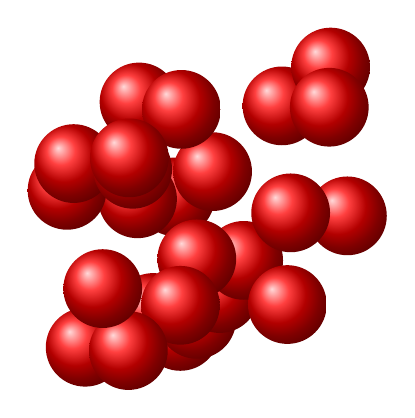
\begin{tikzpicture}
  \foreach \z in {0,...,24}{
    \shade[ball color=red] ({rand*1.5},{rand*1.5},{rand*1.5}) circle(0.5);
  }
\end{tikzpicture}
\subcaption{} \label{fig:M3}
\end{subfigure}
\par\bigskip
\caption{Schematic representation of different degrees of ordered structures, where (a) is a crystalline of a simple cubic lattice, (b) is a polycrystalline hexagonal lattice, and (c) is an amorphous lattice.}
\label{fig:crystalstructure}
\end{figure}


Solid materials, like plastic bottles, are formed by densely packed atoms. These atoms can randomly occur through the material without any long-range order or periodically ordered in small regions of the material, which would categorize the material as either an \textit{amorphous solid} or \textit{polycrystalline solid}. %, or the atoms can be periodically ordered in small regions of the materials,  %Amorphous solids are frequently used in gels, glass and polymers \cite{BenStreetman2015}.
%However, the atoms can also be periodically ordered in small regions of the material, classifying the material as a \textit{polycrystalline solid}.
%All ceramics are polycrystalline with a broad specter of applications ranging from kitchen-porcelain to orthopedical bio-implants \cite{Renganathan2018}.
A third option is to have these atoms arranged with infinite periodicity, making the material a \textit{crystalline solid} or more commonly named a \textit{crystal}. The three options are visualised in figure \ref{fig:crystalstructure}. Hereon, we will focus on crystalline solids.

The periodicity in a crystal is defined in terms of a symmetric array of points in space called the \textit{lattice}, which can be simplified as either a one-dimensional array, a two-dimensional matrix or a three dimensional vector space, depending on the material. At each lattice point we can add an atom to make an arrangement called a \textit{basis}. The basis can be one atom or a cluster of atoms having the same spatial arrangement. Every crystal has periodically repeated building blocks called \textit{cells} representing the entire crystal. The smallest cell possible is called a \textit{primitive cell}, but such a cell only allows lattice points at its corners and it is often quite rigid to work with when the structure becomes complex. As a solution, we will consider the \textit{unit cell}, which allows lattice points on face centers and body centers.

One example of a crystal structure is the perovskite structure. Compounds with this structure are characterized by having an $ABX_3$ stoichiometry whose symmetri belong to one of 15 space groups identified by Lufaso \& Woodward \cite{Lufaso2001}, such as the cubic, orthorombic and tetragonal. For our purpose, we will be looking into when the X atom is oxygen, and refer to the oxygen-perovskite $ABO_3$. The A atom is nine- to 12-fold coordinated by oxygen, while the B atom is sixfold coordinated by oxygen, and the $BO_6$ octahedra are connected to the corners in all three directions as visualized in figure \ref{fig:perovskite}.

\begin{wrapfigure}{r}{0.5\textwidth}
  \centering
  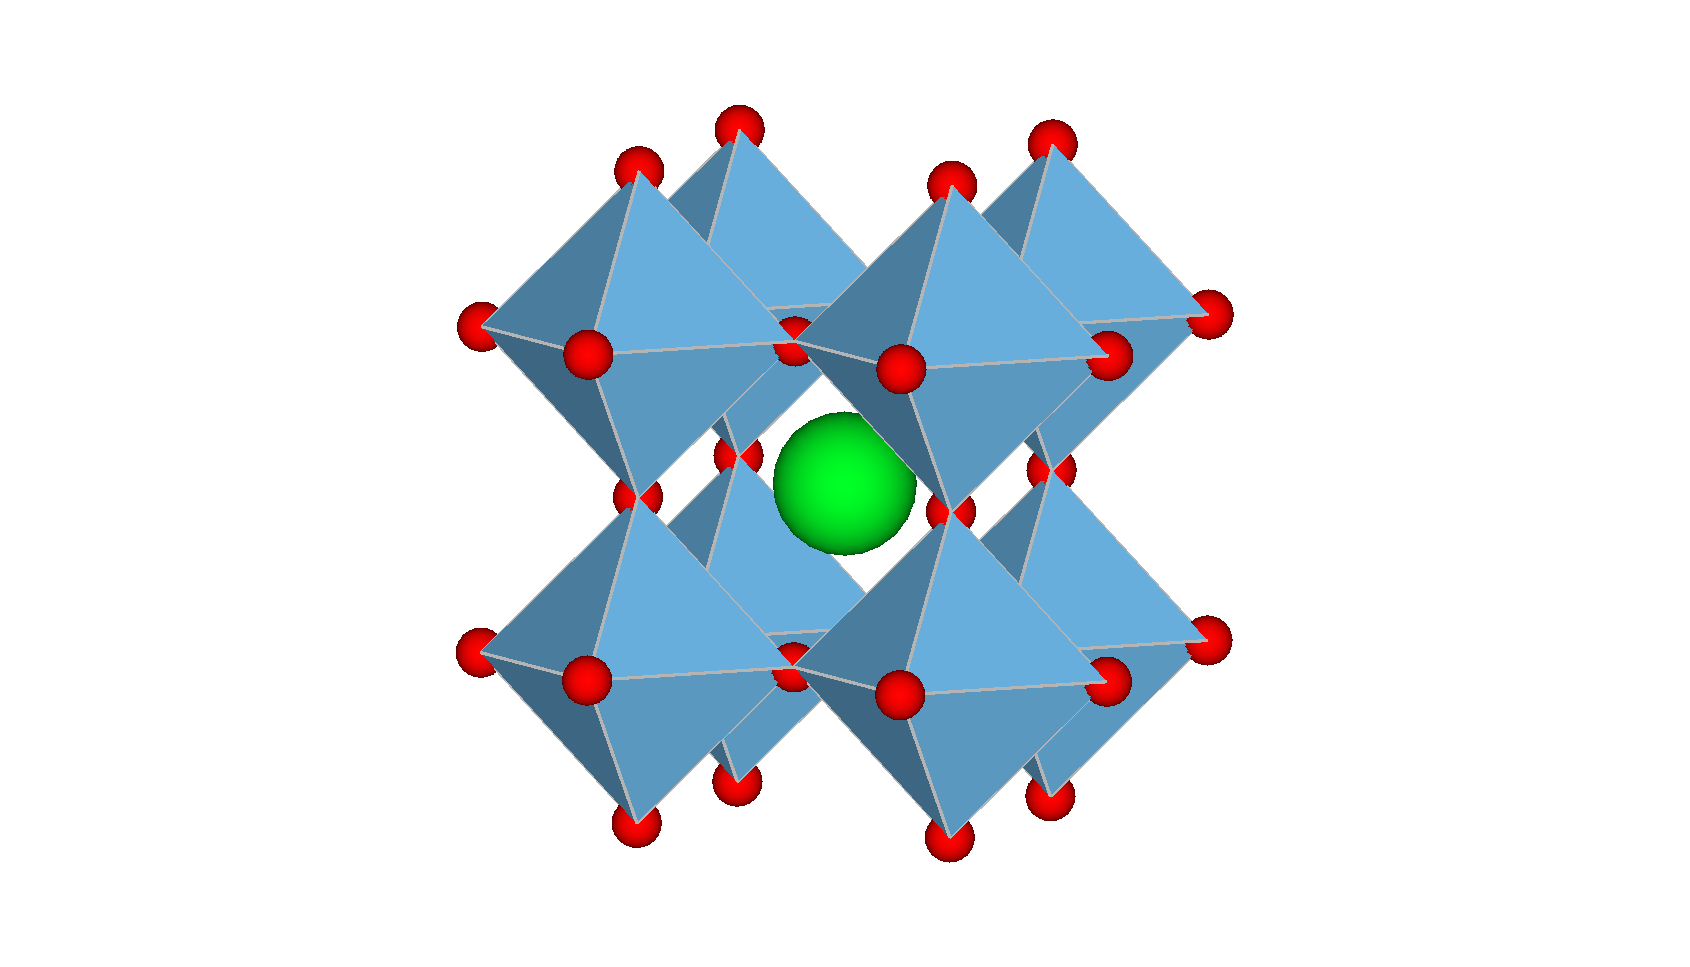
\includegraphics[width=0.48\textwidth]{theory/figures/SrTiO3_mp-5229_primitive.pdf}
  \caption{A crystal structure of SrTiO$_3$ which is a cubic perovskite. The red atoms are oxygen, whereas the green atom is strontium, and inside every corner-sharing BO$_6$ octahedral unit is a titanium atom.}
  \label{fig:perovskite}
\end{wrapfigure}

The motivation behind the research on perovskites is related to the large amount of available ABO$_3$ chemistries, where a significant portion of these take the perovskite structure. Perovskites have a broad specter of applications, ranging from high-temperature superconductors \cite{Bednorz1988} and ionic conductors \cite{Boivin1998} to multiferroic materials \cite{Cheong2007}. Additionally, adding a perovskite-type compound to solar cells has reportedly resulted in higher performance efficiencies while being cheap to produce and simple to manufacture \cite{IbnMohammed2017, Chen2014}. However, this includes the use of hybrid organic-inorganic compounds and excludes the use of oxygen.

%Point defects are the type of defect that can be utilised in generating a qubit, thus being a special interest for this thesis. They can arise as either a vacancy in the lattice, interstitial placement inbetween lattice sites, or as a substitution of an existing atom in the lattice.

%Her kan jeg skrive videre om NV -1 strukturen og defekten, da den blir brukt senere.


Isolated atoms have distinct energy levels, where the Pauli exlusion principle \cite{Pauli1925} states for fermions that each energy level can at most accomodate two electrons of opposite spin. In a solid, the discrete energy levels of the isolated atom spread into continuous energy bands since the wavefunctions of the electrons in the neighboring atoms overlap. Hence, an electron is not neccessarily localized at a particular atom anymore. This is exemplified as every material has a unique band structure, similar to every human having their unique fingerprint.

Knowing which energy bands are occupied by electrons is the key in understanding the electrical properties of solids. The highest occupied electron band at $0$ K is called the valence band (VB), while the lowest unoccupied electron band is called the conduction band (CB). The energy gap between the maximum VB and the minimum CB is known as the band gap, and its energy is denoted as $E_g$. If a material can be classified as a semiconductor depends on the band gap and the electrical conductivity. As an example, Silicon is commonly thought of as a semiconductor, and has a band gap of about $1.12$ eV at $275$ K \cite{Martienssen2005}.


\begin{wrapfigure}{r}{0.35\textwidth}
  \begin{minipage}{\linewidth}
    \centering\captionsetup[subfigure]{justification=centering}
  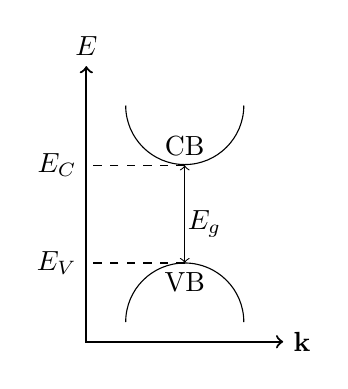
\begin{tikzpicture}[scale=1]
      \draw [<->,thick] (0,3.5) node (yaxis) [above] {$E$}
          |- (2.5,0) node (xaxis) [right] {$\textbf{k}$};
      \draw (0.5,0.25) arc(180:0:0.75cm);
      \draw (2.0,3.0) arc(0:-180:0.75cm);
      \coordinate (VB) at (1.25,1.0);
      \coordinate (CB) at (1.25,2.24);
      \draw[<->] (CB) node[above] {CB}
        -| (VB) node[below] {VB};
      \draw[dashed] (VB) -- (0,1.0) node[left]{$E_V$};
      \draw[dashed] (CB) -- (0,2.24) node[left]{$E_C$};
      \node at (1.5,1.5) {$E_g$};
  \end{tikzpicture}
  \subcaption{}
  \label{fig:directbandgap}
  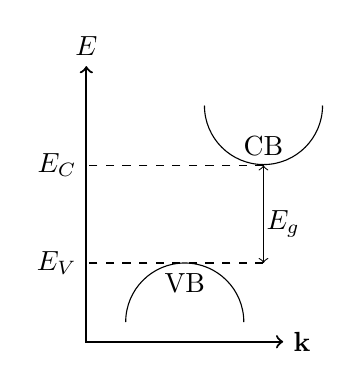
\begin{tikzpicture}[scale=1]
      \draw [<->,thick] (0,3.5) node (yaxis) [above] {$E$}
          |- (2.5,0) node (xaxis) [right] {$\textbf{k}$};
      \draw (0.5,0.25) arc(180:0:0.75cm);
      \draw (3.0,3.0) arc(0:-180:0.75cm);
      \coordinate (VB) at (2.25,1.0);
      \coordinate (CB) at (2.25,2.24);
      \draw[<->] (CB) node[above] {CB}
        -| (VB);
      \draw[dashed] (VB) -- (0,1.0) node[left]{$E_V$};
      \draw[dashed] (CB) -- (0,2.24) node[left]{$E_C$};
      \node at (2.5,1.5) {$E_g$};
      \node at (1.25,0.75) {VB};
  \end{tikzpicture}
  \label{fig:indirectbandgap}
  \subcaption{}
  \end{minipage}
  \caption{A schematic drawing of a (a) direct bandgap and an (b) indirect bandgap.}
\end{wrapfigure}


To be able to accelerate electrons in a solid using an electrical field, they must be able to move into new energy states. At $0$ K, the entire valence band of a semiconductor is full with electrons and there are no available states nearby, making it impossible for current to flow through the material. This can be solved by using either thermal or optical energy to excite electrons from the valence band to the conduction band, in order to \textit{conduct} electricity. At a given temperatuer, some semiconductors will have electrons excited to the conduction band solely from thermal energy matching the energy band gap \cite{BenStreetman2015}.

In some scenarios, thermal or optical energy is not sufficient for an excitation since the energy bands are also dependent on the crystal momentum. A difference in the momentum of the minimal-energy state in the conduction band and the maximum-energy state in the valence band results in an \textit{indirect bandgap} as seen in figure \ref{fig:indirectbandgap}. If there is no difference at all, the material has a \textit{direct bandgap}, which is visualized in figure \ref{fig:directbandgap}.

Electrons in semiconductor materials can be described according to the Fermi-Dirac distribution
\begin{align*}
  f(E) = \frac{1}{1+e^{(E-E_F)/kT}},
\end{align*}
where $k$ is Boltzmann's constant, $T$ is temperature, $E$ is the energy and $E_F$ is the Fermi level. The Fermi-Dirac distribution gives the probability that a state will be occupied by an electron, and at $T=0$ K, every energy state lower than $E_F$ is occupied by electrons while the opposite is true for energy states above $E_F$ \cite{BenStreetman2015}.

\subsection{Point defects in semiconductors}

In real life, a perfect crystal without any symmetry-breaking flaw does not exist. These flaws are known as defects and can occur up to three dimensions. An example one-dimensional defect is known as a \textit{line defect}, while two dimensional defects can be \textit{planar defects}, and in three dimensions we have \textit{volume defects}. Lastly, defects can also occur in zero dimensions and are then termed \textit{point defects}. Point defects normally occur as either vacancies, interstitially placed atoms inbetween lattice sites (called interstitials) or as substitution of another existing atom in the lattice.

Defects can greatly influence both the electronic and optical propertires of a material. A substitional defect may be an unintentionally introduced impurity or an antisite, but they can also be intentionally inserted, an approach normally known as \textit{doping}. Doping can result in an excess of electrons or holes, making the semiconductor either an n- or p-type, respectively. Consequently, the semiconductor will have energy levels in the (forbidden) band gap that originates from the defects. If the energy levels introduced are closer than $ \sim 0.2$ eV to the band egdes, they are termed \textit{shallow} defects.

Shallow defects can contribute with either excess electrons to the conduction band, or excess holes to the valence band. However, the induced charge carriers (electrons or holes) interact strongly with the band egdes, resulting in a delocalized wavefunction.% regarding the position in the lattice. %For the latter scenario, shallow defects are commonly labelled as \textit{dopants}.

For the opposite case, if the energy levels rests closer to the middle of the semiconductor's gap, the introduced defects are known as \textit{deep level} defects. Deep levels may be of intrinsic or extrinsic origin, %normally occur due to either dangling bonds or impurities,
and have highly localized electron wavefunctions. This might assure the isolation required for long coherence times, which is an appealing promise in quantum technological advances.

Deep levels can be unfortunate in semiconductors since they can interact with the charge carriers, potentially modifying the desired electronic or optical property of the material. Deep level defects can function as electron-hole recombination centers, or to trap charge carriers, yielding the commonly used name deep level \textit{traps}. Both of the given situations results in a lower concentration of charge carriers, which showcase why deep levels normally are unwanted in semiconductor devices. However, deep level defects may be beneficially used in quantum technology. %show extraordinary properties in quantum technology due to their ability to ensure isolation and preserve coherence.

\subsection{Optical defect transitions}

Optical transitions refers to excitation or de-excitation of charge carriers due to either emission or absorption of electromagnetic radiation.%, and can be done with a laser light or electron beam.
Figure \ref{fig:configurationcoordinate} represents a configuration coordinate (CC) diagram of a defect transition. The y-axis is the energy $E$, while the x-axis is the configuration coordination $Q$, which represents the atomic displacement from the equilibrium position $Q_{GS}$. The lowest point in the lower parabola is known as the ground state (GS) configuration $Q_{GS}$, which is the most stable atomic position, while for the upper parabola it is known as the excited state configuration $Q_{ES}$. The dotted lines represent vibronic excitations to the energy of the ground state $Q_{GS}$ for the lower parabola, while it represents $Q_{ES}$ for the higher parabola.


\begin{figure}[!ht]
  \centering
  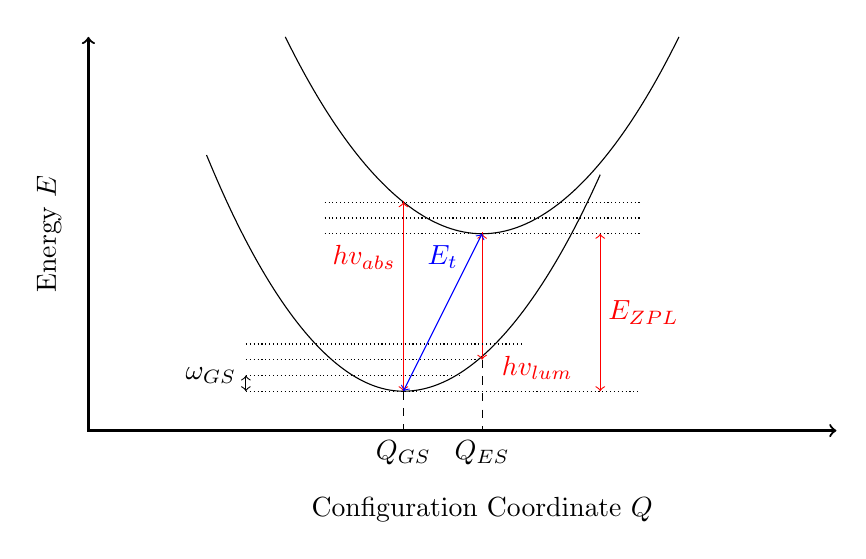
\begin{tikzpicture}[scale=1]
      \draw [<->,thick] (0,5.0) node (yaxis) [left] {}
          |- (9.5,0) node (xaxis) [below left] {};

      \draw (1.5,3.5) parabola bend (4,0.5) (6.5,3.25);
      \draw (2.5,5.0) parabola bend (5.0,2.5) (7.5,5.0);
      \node[rotate=90] at (-0.5,2.5){\text{Energy} $E$};

      \draw[<->, color=red] (4.0,2.9)
        -| (4.0,0.50);

      \draw[<->, color=red] (5.0,2.5)
          -| (5.0,0.9);

      \draw[<->, color=blue] (4.0,0.50) -- (5.0,2.5);
      \node[color=red] at (3.5,2.2) {$hv_{\text{abs}}$};
      \node[color=blue] at (4.5,2.2) {$E_t$};
      \node[color=red] at (5.7,0.8) {$hv_{\text{lum}}$};

      \draw[densely dotted] (2.0,0.5) -- (7.0,0.5);
      \draw[densely dotted] (2.0,0.7) -- (4.75,0.7);
      \draw[densely dotted] (2.0,0.9) -- (5.0,0.9);
      \draw[densely dotted] (2.0,1.1) -- (5.5,1.1);

      \draw[<->] (2.0,0.50) -- (2.0,0.7) node[left]{$\hslash \omega_{GS}$};

      \draw[densely dotted] (3.0,2.5) -- (7.0,2.5);
      \draw[densely dotted] (3.0,2.7) -- (7.0,2.7);
      \draw[densely dotted] (3.0,2.9) -- (7.0,2.9);

      \draw[<->, color=red] (6.5,0.50) -- (6.5,2.5);
      \node[color=red] at (7.05,1.5) {$E_{ZPL}$};

      \draw[dashed] (4.0,0.50) -- (4.0,0.0) node[below]{$Q_{GS}$};
      \draw[dashed] (5.0,0.9) -- (5.0, 0) node[below]{$Q_{ES}$};

      \node at (5.0,-1.0){\text{Configuration Coordinate} $Q$};
      %\draw[dashed] (VB) -- (0,1.0) node[left]{$E_V$};
      %\draw[dashed] (CB) -- (0,2.24) node[left]{$E_C$};
      %\node at (2.5,1.5) {$E_g$};
      %\node at (1.25,0.75) {VB};
  \end{tikzpicture}
  \caption{A schematic representation of a configuration coordination diagram based on Ref. \cite{Pelant2012}.}
  \label{fig:configurationcoordinate}
\end{figure}


\noindent The optical transitions in figure \ref{fig:configurationcoordinate} are marked with red arrows. During slow transitions, such as during thermodynamic defect transitions, the original configuration have time to rearrange due to phonon vibrations. This is schematically drawn as the blue arrow, where the energy $E_t$ equals the ionization energy or the position of the defect level. Optical transitions, on the other hand, are marked in red and occur in a short time range such that the original configuration does not change. They can appear in the exchange of charge carriers with the band egdes, and in a defect's internal excited state, with the latter scenario being most relevant for this thesis.

Consider a defect that rests in the ground state configuration $Q_{GS}$. Suddenly, it absorbs a photon with energy $h v_{\text{abs}}$ and occupies an excited vibronic state of the upper parabola after a vertical transition. Through lattice reconfigurations, the defect will move towards the bottom of the upper parabola, also known as $Q_{ES}$. Eventually, it will relax to the lower parabola by emitting a photon with energy $h v_{lum}$, also known as a zero-phonon line (ZPL) of energy $E_{ZPL}$. On the other hand, any transitions between vibronic excitation levels are phonon-related. How strong the electron-phonon interaction is can be quantified by the Huang-Rhys factor $S$ \cite{Huang1950}. If the two parabolas in figure \ref{fig:configurationcoordinate} have the same configuration of $Q$, emission into the ZPL is enabled and $S\sim 0$. The stronger the coupling, the smaller amount of emission in the ZPL.

The optical properties of a host material can be greatly influenced by defects, in particular the ES to GS transition that can occur in a defect, as discussed for figure \ref{fig:configurationcoordinate}. If the defect were to fascilitate the emission of single photons with a detectable time inbetween together with a distinguishable ZPL, the defect would be referred to as a single photon source (SPS). The criteria for SPS are not met in many materials or defect systems, since charge-state transitions often comprise interactions with either the VB or the CB. Thus, most SPSs' GS and ES levels are situated within the band gap of a host material. Consequently, mostly wide-band gap semiconductors are used as host materials for SPSs.

\section{Semiconductor candidates for quantum technology}

The properties of point defects are promising in a quantum technological perspective. We have seen that point defects can fasciliate deep energy levels within the band gap of the semiconductor, and provide isolation in the solid-state matrix as a result from a high degree of localization of the defect orbitals. If the host material have a small spin-orbit coupling, it could provide long coherence times for a deep level trap in localized and high-spin states. Additionally, point defects have the potential to be single-photon sources, giving rise to sharp and distinguishable optical transitions, where a significant amount of the emission can be of the energy $E_{ZPL}$. This is in particular seen in wide-bandgap semiconductors, and combined with a weak electron-phonon interaction, can have the capacity to be fabricated as a high-fidelity SPS with a significant ZPL part.

In this section we will provide specific examples of a variety of promising candidates, and what properties they possess that makes them auspicious. Additionally, we will briefly mention what the challenges with the candidates are, and why it is important to explore other viable options.

\subsection{Diamond - the benchmark material for QT}
\label{diamond}

\begin{figure}[ht!]
  \centering
\begin{subfigure}{1.0\linewidth}
\centering
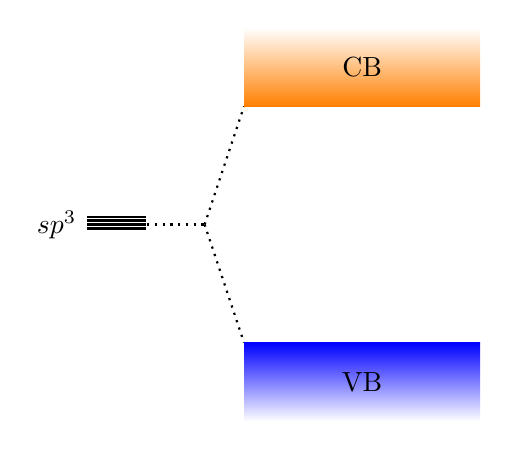
\begin{tikzpicture}

  \atom[name=C, color=orange, pos={(-2,0)},scale=0.5]{
    gray/45/45/0,
    gray/315/315/0,
    gray/225/225/0,
    gray/135/135/0}

  \draw[thick,-] (-1.25,-4) -- (-2.0,-4) node[anchor=east]{$sp^3$};
  \draw[thick,-] (-1.25,-3.95) -- (-2.0,-3.95);
  \draw[thick,-] (-1.25,-4.05) -- (-2.0,-4.05);
  \draw[thick,-] (-1.25,-3.90) -- (-2.0,-3.90);

  \draw[thick, dotted] (-1.23,-4) -- (-0.5,-4);
  \draw[thick, dotted] (-0.5,-4) -- (0,-5.5);
  \draw[thick, dotted] (-0.5,-4) -- (0,-2.5);

  %\node at (1.5,1.5) {$E_g$};
  %\draw (0,-1.5) -- (2,-1.5) -- (2,-2) -- (0,-2) -- (0,0);
  \shade[top color=white,bottom color=orange] (0,-2.5) rectangle (3.0,-1.5) node[pos=.5] {CB};
  \shade[top color=blue,bottom color=white] (0.,-6.5) rectangle (3.0,-5.5) node[pos=.5] {VB};

  \atom[name=C, color=orange, scale=0.5]{
    gray/45/45/0,
    gray/315/315/0,
    gray/225/225/0,
    gray/135/135/0}
  \atom[name=C, color=orange, pos={(0.75,0.75)},scale=0.5]{
    gray/45/45/0,
    gray/315/315/0,
    gray/225/225/0,
    gray/135/135/0}
  \atom[name=C, color=orange, pos={(1.5,0)},scale=0.5]{
    gray/45/45/0,
    gray/315/315/0,
    gray/225/225/0,
    gray/135/135/0}
  \atom[name=C, color=orange, pos={(0.75,-0.75)},scale=0.5]{
    gray/45/45/0,
    gray/315/315/0,
    gray/225/225/0,
    gray/135/135/0}
  \atom[name=C, color=orange, pos={(2.25,0.75)},scale=0.5]{
    gray/45/45/0,
    gray/315/315/0,
    gray/225/225/0,
    gray/135/135/0}
  \atom[name=C, color=orange, pos={(2.25,-0.75)},scale=0.5]{
    gray/45/45/0,
    gray/315/315/0,
    gray/225/225/0,
    gray/135/135/0}
  \atom[name=C, color=orange, pos={(3.0,0)},scale=0.5]{
      gray/45/45/0,
      gray/315/315/0,
      gray/225/225/0,
      gray/135/135/0}

\end{tikzpicture}
\subcaption{} \label{fig:diamond structure}
\end{subfigure}%

\begin{subfigure}{1.0\linewidth}
\centering
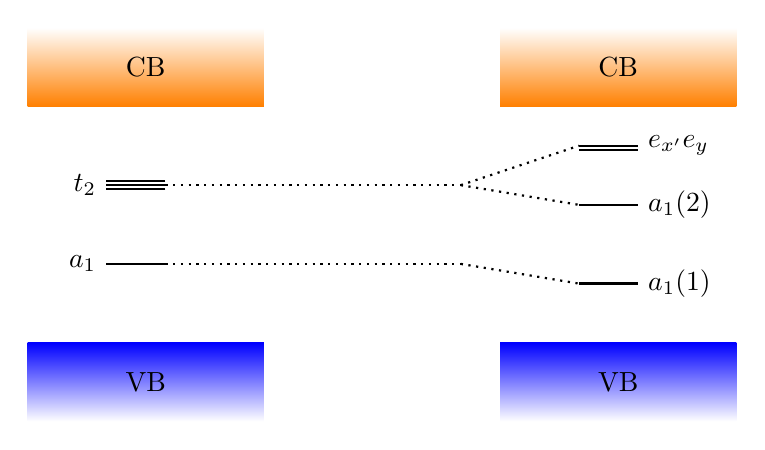
\begin{tikzpicture}

  \shade[top color=white,bottom color=orange] (0.-7,-2.5) rectangle (3.0-7,-1.5) node[pos=.5] {CB};
  \shade[top color=blue,bottom color=white] (0.-7,-6.5) rectangle (3.0-7,-5.5) node[pos=.5] {VB};

  \draw[thick,-] (1.75-7,-4.5) -- (1.0-7,-4.5) node[anchor=east]{$a_1$};
  \draw[thick,-] (1.75-7,-3.5) -- (1.0-7,-3.5) node[anchor=east]{$t_2$};
  \draw[thick,-] (1.75-7,-3.55) -- (1.0-7,-3.55);
  \draw[thick,-] (1.75-7,-3.45) -- (1.0-7,-3.45);

  \atom[name=C, color=orange, pos={(0-7,0)}, scale=0.5]{
    gray/45/45/0,
    gray/315/315/0,
    gray/225/225/0,
    gray/135/135/0}
  \atom[name=C, color=orange, pos={(0.75-7,0.75)},scale=0.5]{
    gray/45/45/0,
    red/315/315/0,
    gray/225/225/0,
    gray/135/135/0}
  \atom[name=v, color=gray, pos={(1.5-7,0)},scale=0.5]{}
  \atom[name=C, color=orange, pos={(0.75-7,-0.75)},scale=0.5]{
    red/45/45/0,
    gray/315/315/0,
    gray/225/225/0,
    gray/135/135/0}
  \atom[name=C, color=orange, pos={(2.25-7,0.75)},scale=0.5]{
    gray/45/45/0,
    gray/315/315/0,
    red/225/225/0,
    gray/135/135/0}
  \atom[name=C, color=orange, pos={(2.25-7,-0.75)},scale=0.5]{
    gray/45/45/0,
    gray/315/315/0,
    gray/225/225/0,
    red/135/135/0}
  \atom[name=C, color=orange, pos={(3.0-7,0)},scale=0.5]{
      gray/45/45/0,
      gray/315/315/0,
      gray/225/225/0,
      gray/135/135/0}

    \shade[top color=white,bottom color=orange] (0.-1.,-2.5) rectangle (3.0-1.0,-1.5) node[pos=.5] {CB};
    \shade[top color=blue,bottom color=white] (0.-1.,-6.5) rectangle (3.0-1.0,-5.5) node[pos=.5] {VB};

    \atom[name=C, color=orange, pos={(0.-1.,0)}, scale=0.5]{
      gray/45/45/0,
      blue/315/315/0,
      gray/225/225/0,
      gray/135/135/0}
    \atom[name=C, color=orange, pos={(0.75-1,0.75)},scale=0.5]{
      gray/45/45/0,
      red/315/315/0,
      gray/225/225/0,
      gray/135/135/0}
    \atom[name=v, color=gray, pos={(1.5-1,0)},scale=0.5]{}
    \atom[name=N, color=green!95, pos={(0.75-1,-0.75)},scale=0.5]{
      blue/45/45/0,
      blue/315/315/0,
      blue/225/225/0,
      blue/135/135/0}
    \atom[name=C, color=orange, pos={(2.25-1,0.75)},scale=0.5]{
      gray/45/45/0,
      gray/315/315/0,
      red/225/225/0,
      gray/135/135/0}
    \atom[name=C, color=orange, pos={(2.25-1,-0.75)},scale=0.5]{
      gray/45/45/0,
      gray/315/315/0,
      gray/225/225/0,
      red/135/135/0}
    \atom[name=C, color=orange, pos={(3.0-1,0)},scale=0.5]{
        gray/45/45/0,
        gray/315/315/0,
        gray/225/225/0,
        gray/135/135/0}

    \draw[thick, dotted] (1.75-7,-3.5) -- (-1.5,-3.5);
    \draw[thick, dotted] (-1.5,-3.5) -- (0,-3.0);
    \draw[thick, dotted] (-1.5,-3.5) -- (0,-3.75);

    \draw[thick,-] (1.0-1,-3.0) -- (1.75-1,-3.0) node[anchor=west]{$e_{x'}e_y$};
        \draw[thick,-] (1.75-1,-3.05) -- (1.0-1,-3.05);
    \draw[thick,-] (1.0-1,-3.75) -- (1.75-1,-3.75) node[anchor=west]{$a_1(2)$};

    \draw[thick, dotted] (1.75-7,-4.5) -- (-1.5,-4.5);
    \draw[thick, dotted] (-1.5,-4.5) -- (0,-4.75);
    \draw[thick,-] (1.0-1,-4.75) -- (1.75-1,-4.75) node[anchor=west]{$a_1(1)$};

\end{tikzpicture}
\subcaption{} \label{fig:defect diamond structure}
\end{subfigure}
\par\bigskip
\caption{A schematic representation of the electronic structure of the NV$^{-1}$ defect in a tetrahedrally coordinated semiconductor, exemplified by diamond. Figure used from Ref. \cite{Gordon2013}.}
\label{fig: diamond electronic structure}
\end{figure}


The most studied point defect system is the nitrogen-vacancy ($NV^{-1}$) in diamond. Figure \ref{fig: diamond electronic structure} schematically shows the negative charge state of the electronic structure in diamond. Panel \ref{fig:diamond structure} shows the electronic states that correspond to the difference for an isolated atom and a lattice of atoms, as a superposition of $sp^3$ orbitals that generates valence and conduction bands. In panel \ref{fig:defect diamond structure}, a vacancy has been created by removing a carbon atom, and the four orbitals interact with each other resulting in two new states with $a_1$ and $t_2$ symmetry due to dangling bonds. Substituting a carbon atom with a nitrogen atom further splits the $t_2$-states into two new states. The states $a(1)$ and $e_{x'}e_y$ are of importance, as they are the GS and the ES of the qubit defects, respectively. Here, an optical spin-conserving transition can occur due to a laser light of correct wavelength \cite{Gordon2013}, as exemplified from the discussion from the last section.

\noindent The nitrogen-vacancy in diamond is a prominent single-photon source up to room temperatures. This involves initializing, manipulating and reading out of the qubit state using optical and electric excitations, and electric and magnetic fields \cite{Gordon2013}. The potential qubit system have promising applications in quantum- communication and computation, with a demonstrated entanglement between two NV center spins that are separated by $3$ m \cite{Bernien2013}. Nevertheless, perhaps the most propitious application can be seen in quantum sensing as high-sensivity magnetometer with nanoscale resolution \cite{Taylor2008}.

Unfortunately, the NV-center display several drawbacks that may limit the use in quantum communication and computation. In particular, the amount of emission into the zero-phonon line is only $4 \%$ at $6$ K \cite{Barclay2011}. The emission of the qubit center is not completely compatible with current optical fiber technologies, since the emission is in the red wave-length specter. Additionally, fabricating materials of diamond is far from unchallenging and serves as a signficant incentive to find other promising qubit candidates.

\subsection{Qubit material host requirements}
\label{ssec:qubit-material-host-requirements}
Therefore, we turn to the search of other QT compatible hosts that offers similar capabilities, but that are more user-friendly. In particular, we need to search for new promising materials that can host a potential point defect. \citeauthor{Weber2010} \cite{Weber2010} proposed in 2010 four criteria that should be met for a solid-state semiconductor material hosting a qubit defect, whereas some of the criteria has already been discussed. An ideal crystalline host should have \cite{Weber2010}
\begin{itemize}
  \item[(H1)] A wide-band gap to accomodate a deep center.
  \item[(H2)] Small spin-orbit coupling in order to avoid unwanted spin flips in the defect bound states.
  \item[(H3)] Availability as high-quality, bulk, or thin-film single crystals.
  \item[(H4)] Constituent elements with naturally occuring isotopes of zero nuclear spin.
\end{itemize}

%Host candidates that satisfy criteria (H1) and (H2) can be found by studying the electronic structure of the compounds. What tends to happen for defects in semiconductors, is that the electronic states associated with the defect have energies that lie within the (forbidden) band gap of the semiconductor. This is schematically drawn and explained for diamond in figure (\ref{fig: diamond electronic structure}). A large band gap can accomodate multiple highly isolated states and make them confined and isolated from interactions with the environment, which is favorable for longer coherence times. However, the desired band gap depends on the application, since the Fermi level of large band gap materials is challenging to control \cite{Bassett2019}.

\noindent Table (\ref{tab:qubithosts}) lists several material host candidates that exhibit promising band gap capable of accommodating a deep level defect. For example, the spin-orbit splitting is an indication of the strength of the spin-orbit interaction, and is taken at the $\Gamma$ point from the valence-band splitting. A smaller value may indicate less susceptibility to decoherence.

\begin{table}[!ht]
\centering
\noindent\makebox[\textwidth]{
\begin{tabular}{M{2.5cm} M{2.5cm} M{3.0cm} M{4.0cm}}
  \hline
  \hline
  Material & Band gap  $E_g$ (eV) & Spin-orbit splitting $\Delta_{so}$ (meV) & Stable spinless nuclear isotopes? \\
  \hline
  3C-SiC & 2.39 & 10 & Yes \\
  4H-SiC & 3.26 \cite{Neudeck1995} & 6.8 & Yes \\
  6H-SiC & 3.02 & 7.1 & Yes \\
  AlN & 6.13 & 19 \cite{Silveira2005} & No \\
  GaN & 3.44 & 17.0 & No \\
  AlP & 2.45 & 50 \cite{Lawaetz1971} & No \\
  GaP & 2.27 & 80 & No \\
  AlAs & 2.15 & 275 & No \\
  ZnO & 3.44 \cite{Beckers1998} & -3.5 & Yes \\
  ZnS & 3.72 \cite{Kumbhojkar2000} & 64 & Yes \\
  ZnSe & 2.82 & 420 & Yes \\
  ZnTe & 2.25 & 970 & Yes \\
  CdS & 2.48 & 67 & Yes \\
  \hline
  C (Diamond) & 5.5 & 6 & Yes \\
  Si & 1.12 & 44 & Yes \\
  \hline
  \hline
\end{tabular}
}
\caption{Table taken from \citeauthor{Gordon2013} \cite{Gordon2013} that lists a number of tetrahedrally coordinated hosts whose band gaps are larger than $2.0$ (eV), and compares it to diamond and Si. All experimental values are from Ref. \cite{Martienssen2005}, except for where explicity cited otherwise. }
%For materials where more than one structure is stable in room temperature, the most dominant room-temperature phase's band parameters are chosen.}
\label{tab:qubithosts}
\end{table}

Criterion (H3) is important for scalability and further potential for a large-scale fabrication. The given candidate hosts provided in table (\ref{tab:qubithosts}) can all be grown as single crystals, but with varying quality and size.

\noindent Normally, nuclear spin is a major source of decoherence for all semiconductor-based quantum technologies. This would exclude the use of all elements in odd groups in the periodic table, since these elements exhibit nonzero nuclear spin. As a result, the spin-coherence time of a paramagnetic deep center \cite{Weber2010} might increase. However, nuclear spin can also induce additional quantum degrees of freedom for applications in the proper configuration \cite{Bassett2019}. Therefore, criterion (H4) is not a strict requirement but is a general recommendation for reducing decoherence time.  %Therefore, we will not completely exclude all nonzero nuclear spin elements from our list.

%In fact, all of the criteria could be regarded as recommendations,

\citeauthor{Weber2010} \cite{Weber2010} use criteria $(H1)-(H4)$ to specifically find analogies to the $NV^{-1}$ center in other material systems, thus leaving the discussion of other criteria out, such as the choice of crystal system. The atomic configuration and crystal structure of a material strongly influences the properties of a defect, since a defect's orbital and spin structure is dependent on its spatial symmetry \cite{Bassett2019}. In particular, it is the point group that decides which multiplicity a given energy level should have \cite{James1976}. A higher defect symmetry group generally facilitates degenerate states, which may give rise to high spin states according to Hund's rules \cite{Bassett2019, Togan2010}. Inversion symmetry in the host crystal can also be beneficial, resulting in reduced inhomogenous broadening and spectral diffusion of optical transitions as a consequence of being generally insensitive to external electric fields \cite{Bassett2019}.

\begin{wrapfigure}{r}{0.6\textwidth}
  \centering
  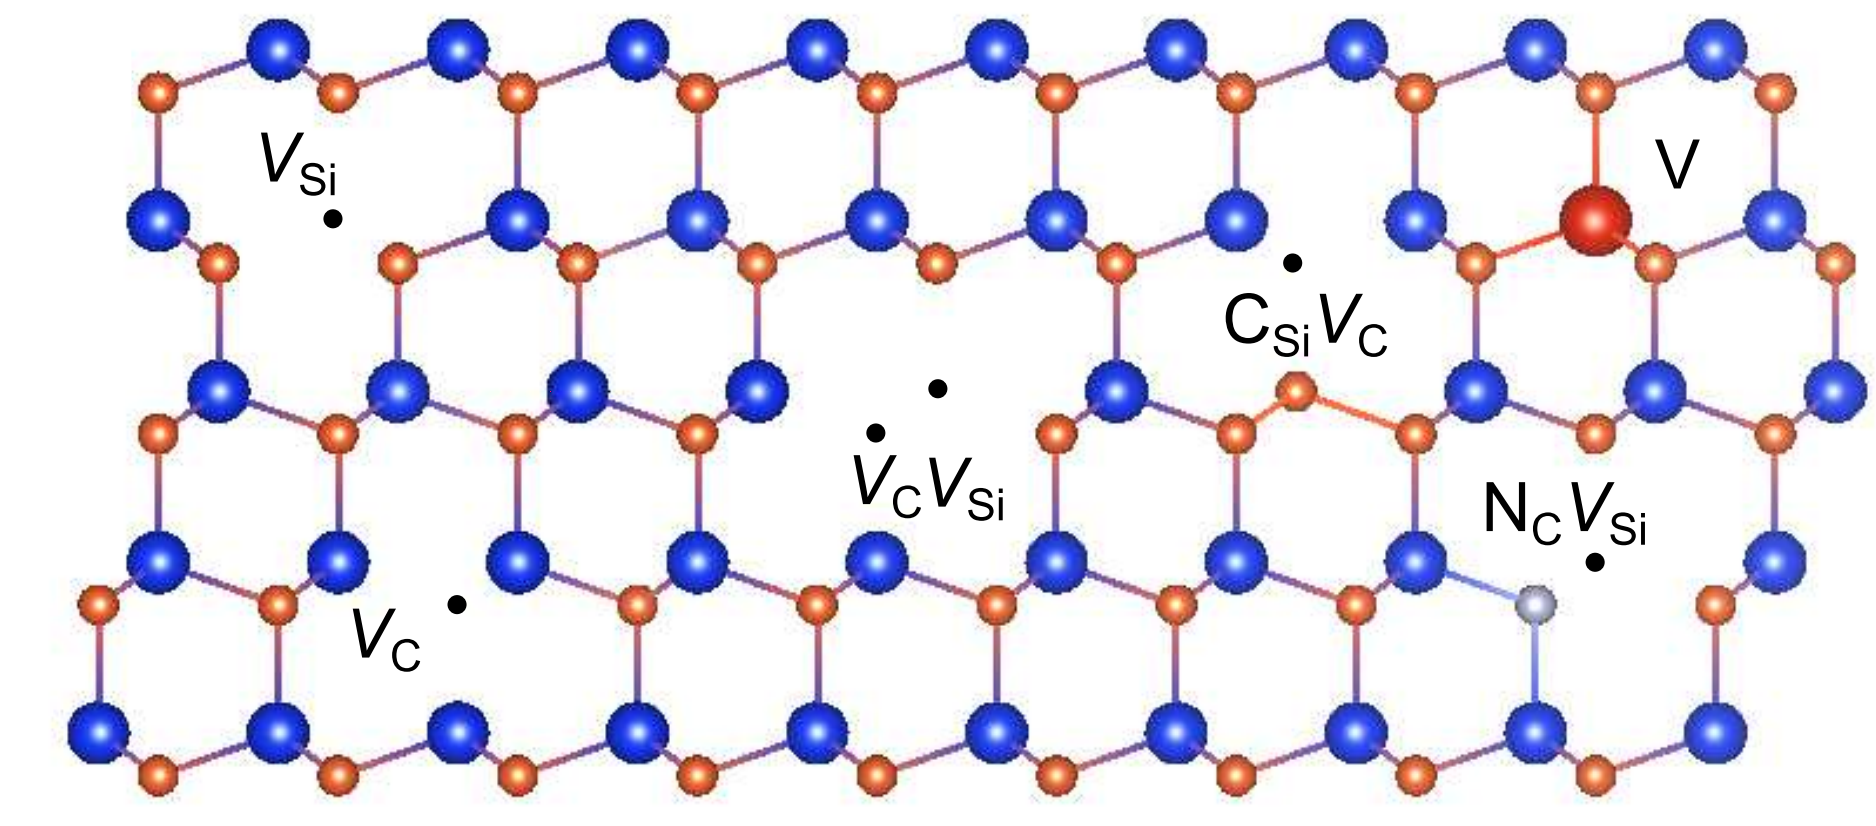
\includegraphics[width=0.6\textwidth]{theory/figures/4H-SiC.png}
  \caption{Schematic illustration of various point defects in 4H-SiC, where Si atoms are blue while C atoms are orange. The illustration includes the point defects Si vacancy ($\text{V}_{\text{Si}}$), C vacancy ($\text{V}_{\text{C}}$), divacancy ($\text{V}_{\text{Si}}\text{V}_{\text{C}}$), carbon antisite-vacancy pair ($\text{C}_{\text{Si}}\text{V}_{\text{C}}$), nitrogen-vacancy ($\text{N}_{\text{C}}\text{V}_{\text{Si}}$) and the vanadium impurity ($\text{V}$). Figure taken from Ref. \cite{Bathen2020}.}
  \label{fig:4H-SiC}
\end{wrapfigure}

\subsection{Silicon carbide}
\label{silicon-carbide}

Silicone carbide (SiC) is an emerging quantum platform that exists in a wide variety of polytypes, with $3C$, 4H and 6H being the most prominent configurations. Several of the polytypes have been demonstrated to host SPEs with a slightly different emitter characteristic, which provides the opportunity to select the desired properties based on the variety of lattice configurations and point defects available \cite{Weber2010, Son2020, Falk2013}. While 3C has a cubic structure, 4H has a hexagonal structure with both hexagonal ($h$) and pseudo-cubic ($k$) lattice sites. 6H is also a hexagonal structure, but with the three orientations that are labelled $h$, $k_1$ and $k_2$. Importantly, SiC in the three varieties experience wide-band gaps, low spin orbit coupling and stable spinless nuclear isotopes \cite{Neudeck1995, Weber2010, Martienssen2005}, as seen from table \ref{tab:qubithosts}. Furthermore, SiC benefits from mature fabrication on the wafer-scale, which checks the last of the four (H1-H4) QT host requirements, marking it as a suitable quantum material platform.


The most studied emitters in SiC include the carbon antisite-vacancy pair $\text{C}_{\text{Si}}\text{V}_{\text{C}}$ that emits in the red, the silicon vacancy $\text{V}_{\text{Si}}$ that emits in the near infra-red, and the divacancy ($\text{V}_{\text{Si}}\text{V}_{\text{C}}$) and the nitrogen-vacancy center ($\text{N}_{\text{C}}\text{V}_{\text{Si}}$) that both emit at near-telecom wavelengths. Thus, the two latter emitters could potentially ease the integration with optic fiber technologies as compared to e.g. the $\text{NV}^{-}$. Additionally, the four different point defects have all been identified as room-temperature SPEs with demonstrated coherent spin control \cite{Widmann2014, }. Illustrations of several configurations of emitters in 4H-SiC are included in figure \ref{fig:4H-SiC}.

\subsection{Alternative promising material hosts}
\label{promising-material-hosts}

Single photon emitters have been observed in other semiconductor materials, however most of the emitters are yet to be identified or are in an early stage of identification. Therefore, specific details about spin- or emission-related structure are yet to be implemented. In this section we will briefly mention recent promising materials for QT.

One immediate potential candidate is silicon, considering the favorable device fabrication processes that are available. It has demonstrated that phosphorous impurities at Si sites can store a quantum state for over $30$ seconds, enabling their use in a potential Kane quantum computer \cite{Zhang2020}. Unfortunately, the P impurity lack any single photon source capabilities. Recently, however, the G-center arising from the carbon-interstitial carbon-substitutional ($\text{C}_{\text{s}}\text{C}_{\text{i}}$) complex was identified as an promising SPE candidate with single photon emissions at telecom wavelength \cite{Redjem2020}.

Other materials that emits individual photons have been detected in other wide-band gap semiconductors, including ZnO, ZnS, GaAs, GaN and AlN \cite{Wang2014, Zhang2020}, although the defect centers responsible for most of the SPE lines have yet to be identified. Additionally, challenges due to the specific materials complicate the implementation of defects for QT. ZnO and ZnS experience a broad emission due to a large photon involvement. GaAs is promising since it has been demonstrated as a SPS, but demonstration of spin manipulation is still in an early phase\cite{Wang2014}. GaN and AlN, on the other hand, are more susceptible to a more narrow emission, where room-temperature SPE has been demonstrated for both GaN \cite{Berhane2018} and wurtzite AlN films \cite{Xue2020}. The defect levels for AlN films have been tentatively assigned to the nitrogen-vacancy and divacancy complexes, but they tend to occur too close to the band edges for any SPE \cite{Zhang2020, Varley2016}.

Recent advances in material growth have enabled the use of hole spin-based semiconductors, such as SiGe quantum wells due to their low disorder and large intrinsic spin-orbit coupling strength \cite{Hardy2019}. Promising materials can also emerge from placing an impurity next to a vacancy. Cation vacancies in possible structures tend to be negatively charged, thus the impurities should act as donors. Therefore, the self-activation center in ZnSe can be a promising defect  \cite{Weber2010}, but is still in the early stage of development.

Two-dimensional materials such as hexagonal boron nitride ($h$-BN), MoS$_2$, WSe$_2$ and WS$_2$ are also of interest as quantum platforms \cite{Toth2019, Atatuere2018}. The structure of $h$-BN exists in single- or multilayers, and it has been demonstrated a broad range of stable room-temperature single-photon emitters \cite{Tran2016, Tran2016a}. In WSe$_2$, MoSe$_2$ and WS$_2$, there has been experimentally discovered optical excitation of defects, while also electrical excitation of defects for WS$_2$ \cite{Atatuere2018}. However, secure identification for the source of the emission is yet to be established  \cite{Weston2018, Abdi2018, Atatuere2018}.

\subsection{Associated challenges with material host discovery}

The idea of finding new potential host candidates to utilise point defects in QT is challenging. Recall, we have made four criteria that deals with the requirements; (H1) band gaps, (H2) spin-orbit coupling, (H3) availability and (H4) spin-zero isotopes, but more criterias may be needed and the excisting ones refined.%we have no knowledge of if there should be more criteria or to what extent a criteron needs to be fulfilled.
What we do know is that there are major advantages if materials exhibit properties such as isolation in the lattice and weak electron-photon interaction, however, the process to provide any quantity of measurements are through approximations and material-specific properties. These approximations does not neccessarily capture quantum properties well.

Furthermore, the identified candidates constitues an immensely selective group of only a handful potential hosts which have been discovered by serendipitet. As an example, most known potential hosts are elemental (unary) or binary compounds. This is probably due to the increasing complexity dealing with an additional level of interactions in the lattice. Therefore, there are reasons to believe that many potential hosts are yet to be discovered, which serves as a motivation for studies involving exploratory research for new candidates.

%and quantum technology can still be regarded as a preliminary phase of development.

%It is not to avoid that quantum technology is in its preliminary phase of development. Therefore, there are reasons to believe that many potential hosts are yet to be discovered.

%The author is not aware of any work with the objective of identifying candidate hosts, however, similar work has recently been published.

%However, it is not to avoid that both quantum  hardware and -software is in its preliminary phase of development, and it will be interesting to follow up the progression the following years.


\clearpage
